\documentclass[aps,pra,twocolumn,superscriptaddress,floatfix,longbibliography]{revtex4-2}

\usepackage{amsmath,amssymb}
\usepackage{graphicx}
\usepackage{bm}
\usepackage[colorlinks=true,allcolors=blue]{hyperref}

\newcommand{\Op}{\ensuremath{\mathcal{O}}}
\newcommand{\Za}{\ensuremath{Z\alpha}}
\newcommand{\rd}{\,\mathrm{d}}

\begin{document}

\title{Benchmark Dirac--Debye resonances from a certified exact-structure
spectral method: threshold-amplified spin-symmetry breaking of
autoionization widths}

\author{C.~D.~Reinoso}
\email{cesardanielrrch@gmail.com}
\affiliation{Facultad de Ciencias, Escuela Superior Polit\'ecnica de
Chimborazo (ESPOCH), Riobamba, Ecuador}

\date{\today}

\begin{abstract}
We compute resonances of the radial Dirac equation with the
exponentially screened Coulomb (Yukawa--Debye) potential by two
independent methods: a complex-scaled spectral discretization whose
basis carries the exact Coulomb--Dirac cusp exponent, assembled from
run-time--certified matrices and solved through a mass-shifted
complex-symmetric pencil, and outgoing-wave (Gamow) shooting on the
radial system matched to exact Riccati--Hankel free spinors. The two
methods agree to ten--twelve digits on narrow and moderate resonances,
and the spectral values are stable under rotation angle, basis size and
scale to one part in $10^{10}$. Against the only published Dirac--Yukawa
resonance tables [Shi \emph{et al.}, Few-Body Syst.\ \textbf{55}, 135
(2014)] we reproduce eight of twelve tabulated states at their printed
precision and upgrade them to ten-digit benchmarks; for the narrow
states at their strongest coupling our two methods concur that the
published positions are off by $\sim10^{-2}$ and the published widths
are overestimated by up to two orders of magnitude, a pattern already
visible internally in that work's nonrelativistic-limit comparison; and
we resolve the widths of two near-bound states reported there as zero.
Physically we map the fine-structure (spin-doublet) splitting of the
$2p$ autoionization widths across the full coupling range. Near the
critical screening the splitting is amplified by orders of magnitude:
at fixed reduced screening $\lambda/Z=0.24$ the ratio
$\Gamma_{2p_{3/2}}/\Gamma_{2p_{1/2}}$ grows from $1.000$ at $Z=1$ to
$77.5$ at $Z=80$, and for $Z\gtrsim92$ the $2p_{1/2}$ partner remains
\emph{bound} while the $2p_{3/2}$ autoionizes --- complete breaking of
the near-degeneracy observed at weak coupling and high angular momentum.
Deep in the continuum the same doublet barely splits, identifying the
effect as a threshold phenomenon: the relativistic splitting of the
critical screenings made dynamic. The resonances are born at the
critical screenings of the companion bound-state map with the Wigner
$p$-wave threshold law (measured exponent $1.530$ vs.\ $3/2$), and the
position splitting reverses sign between the threshold and
deep-continuum regimes.
\end{abstract}

\maketitle

\section{Introduction}

Resonances of screened Coulomb systems are a recurring theme across
atomic physics, plasma physics and quantum chemistry: the Yukawa or
Debye--H\"uckel potential models static screening in plasmas and
electrolytes, and the fate of atomic levels as screening
increases---their approach to threshold, dissolution into the continuum,
and the widths of the resulting resonances---controls opacities, line
shapes and ionization balance in dense
environments~\cite{RogersGraboskeHarwood1970,KarHo2007}. The standard
computational tool is complex scaling~\cite{AguilarCombes1971,
BalslevCombes1971,Ho1983,Moiseyev1998}, whose extension to the Dirac
equation has a long history: the mathematical foundation was laid by
\v{S}eba~\cite{Seba1988} and by Balslev and
Helffer~\cite{BalslevHelffer1992}, complex rotation was applied to the
Dirac--Stark problem by Ivanov and Ho~\cite{IvanovHo2004}, a
relativistic $J$-matrix formulation was given by
Alhaidari~\cite{Alhaidari2007}, and the method is in production use in
relativistic mean-field nuclear physics~\cite{GuoCSM2010} and in
complex-scaled relativistic configuration
interaction~\cite{Zaytsev2019}.

For the Dirac--Yukawa problem itself the reference calculation is that
of Shi, Liu, Niu and Guo~\cite{Shi2014}, who applied complex scaling in
a harmonic-oscillator basis, verified their nonrelativistic limit
against the $J$-matrix benchmarks of Alhaidari, Bahlouli and
Abdelmonem~\cite{Alhaidari2008}, and made a physical observation that
frames the present work: the energies and widths of spin doublets ---
fine-structure partners $j=\ell\pm\tfrac12$ --- are approximately
degenerate, preserving a good spin symmetry, in the regime they
studied (high angular momenta $\ell=5$ and $10$). Spin- and
pseudospin-symmetry properties of resonant states are an active topic
in the nuclear-structure community~\cite{LuZhaoZhou2012}.

This paper does two things. First, it establishes benchmark-grade
Dirac--Yukawa resonances by a certified double method: a complex-scaled
spectral discretization built on the exact-structure machinery of a
companion paper~\cite{companionA} --- a Laguerre basis carrying the
analytic cusp exponent $\gamma=\sqrt{\kappa^{2}-(\Za)^{2}}$, exact
generalized Gauss--Laguerre quadrature, run-time certification of the
assembled operator identities, and a mass-shifted pencil that removes
the rest-mass cancellation --- cross-validated against an entirely
independent outgoing-wave shooting calculation. Where the two methods
overlap they agree to ten--twelve digits, which allows us both to
extend the tables of Ref.~\cite{Shi2014} in precision and to adjudicate
them: their narrow states at strong coupling are shifted and their
widths substantially overestimated, an artifact consistent with
harmonic-oscillator basis truncation near threshold and, internally,
with the deviations their own nonrelativistic limit shows against the
$J$-matrix values for precisely such states.

Second, and mainly, it maps what happens to the spin symmetry of
autoionization when the coupling is strong and the states are near
their thresholds --- the atomic regime, opposite in both respects to
that of Ref.~\cite{Shi2014}. The bound-state companion
study~\cite{companionA} found that the critical screenings
$\lambda_{c}(Z,\kappa)$ of fine-structure partners, degenerate
nonrelativistically, split strongly with $\Za$. Here we show the
dynamical counterpart: near threshold the width ratio of the $2p$
doublet grows by orders of magnitude with $\Za$, terminating in a
regime where one partner is still bound while the other autoionizes,
whereas deep in the continuum the same doublet remains nearly
symmetric. The spin-symmetry breaking of resonance widths is thus a
\emph{threshold-amplified} effect, controlled by the relativistic
splitting of the critical screenings.

Hartree atomic units ($\hbar=m=1$, $c=1/\alpha=137.035\,999\,084$) are
used throughout; the potential is $V(r)=-Z e^{-\lambda r}/r$ and
$s=\lambda/Z$ denotes the reduced screening. Energies are binding-form,
$E-c^{2}$, and resonances are written $E_{r}-i\Gamma/2$.

\section{Methods}
\label{sec:methods}

\subsection{Complex-scaled exact-structure discretization}

Under the dilation $r\to re^{i\theta}$ every term of the radial Dirac
coupling operators $\Op_{\pm}=\mp d/dr+\kappa/r$ scales uniformly by
$e^{-i\theta}$, the mass term is unaffected, and the Coulombic part of
the potential scales exactly: the discretized, mass-shifted pencil is
\begin{equation}
H_{\theta}-c^{2}S=
\begin{pmatrix}
e^{-i\theta}V_{d} & c\,e^{-i\theta}K\\[2pt]
c\,e^{-i\theta}K^{T} & e^{-i\theta}V_{d}-2c^{2}S
\end{pmatrix},
\label{eq:pencil}
\end{equation}
built from the \emph{same real, run-time--certified matrices} $K$,
$V_{d}$, $S$ as the Hermitian solver of Ref.~\cite{companionA}; for the
screened potential the smooth factor $e^{-\lambda re^{i\theta}}$ enters
the (converged) quadrature. The matrix is complex symmetric, and two
structural facts carry over from the Hermitian theory exactly. First,
the uniform $e^{-i\theta}$ scaling leaves the indicial equation at the
origin invariant, so $\gamma$ is unchanged and the cusp-adapted basis
remains exact at $r\to0$ under complex scaling. Second, the
singular-value fiber decomposition of the free discretized
operator~\cite{companionT} survives with $\sigma\to\sigma e^{-i\theta}$:
the free spectrum of Eq.~\eqref{eq:pencil} lies \emph{exactly} on the
two rotated branches $\pm\sqrt{c^{4}+c^{2}\sigma_{j}^{2}
e^{-2i\theta}}-c^{2}$, which we verify at the $10^{-10}$ level and
which pins the rotated continua analytically. At $\theta=0$ the solver
reproduces the Hermitian one to $3\times10^{-11}$, and bound states are
$\theta$-independent to $1.4\times10^{-10}$ over
$\theta\in[0.05,0.4]$ (discrete Balslev--Combes).

Resonances are identified by \emph{$\theta$-stability}: eigenvalues of
the rotated-continuum strings move with $\theta$ while resonance
eigenvalues do not, so the resonance is selected as the eigenvalue with
the smallest displacement between two rotation angles. This selector
proved essential: window-based selection can capture
rotated-continuum artifacts that are static in other parameters. Every
tabulated state is computed on a grid of two rotation angles, two basis
sizes and two basis scales, and the maximum spread over the grid is
quoted as its uncertainty; broad states ($\Gamma/E_{r}\gtrsim2$)
require the larger angle pair $\theta=(0.65,0.80)$.

\subsection{Independent validation: Gamow shooting}

The second method shares no code or discretization with the first. The
radial Dirac system is integrated outward from $r_{0}=10^{-8}$ with the
exact indicial direction and a first-order series start, on a
logarithmic grid to $r=1$ (removing the $1/r$ stiffness) and in $r$
beyond; at the matching radius the incoming-wave coefficient is
extracted as the Wronskian of the regular solution with the \emph{exact
free outgoing spinor}, whose upper component is the Riccati--Hankel
function $\hat h_{\ell}(pr)$, $p=\sqrt{E^{2}-c^{4}}/c$, and whose lower
component follows from the Dirac system itself. A complex secant
iteration drives this coefficient to zero (the Siegert condition). The
centrifugal term in the matching spinor is not optional: plane-wave
matching leaves $O(\kappa/pR)$ errors that we measured at the
$10^{-1}$ level before adopting the exact spinors. The method is
limited to $\Gamma\lesssim4$ a.u.: for broader states the outgoing
component dominates the incoming one by more than the double-precision
range at any usable matching radius.

Table~\ref{tab:double} shows the agreement between the two methods:
$4\times10^{-11}$ and $7\times10^{-11}$ relative for the $Z=40$
doublet, $1.1\times10^{-12}$ for the $2p_{3/2}$ resonance at $Z=80$,
with matching-radius stability at the $10^{-10}$ level. In the
nonrelativistic limit ($Z=1$) both channels reproduce the
triple-verified benchmark of the companion nonrelativistic
engine~\cite{companionA} with deviations of the $O(\alpha^{2})$
magnitude and correct sign.

\begin{table}[t]
\caption{Double-method validation: $2p$ resonances $E_{r}-i\Gamma/2$
(a.u.) of $V=-Ze^{-\lambda r}/r$ at $s=\lambda/Z=0.24$. ``Spectral'' is
the $\theta$-stable complex-scaled value; ``shooting'' the independent
Gamow calculation. }
\label{tab:double}
\begin{ruledtabular}
\begin{tabular}{llll}
$Z$, $\kappa$ & spectral & shooting & rel.\ dev.\\
\colrule
40, $+1$ & $2.941245536171$ & $2.941245536305$ & $4\times10^{-11}$\\
         & $-1.355551909824\,i$ & $-1.355551909813\,i$ & \\
40, $-2$ & $3.413196281651$ & $3.413196281388$ & $7\times10^{-11}$\\
         & $-1.806500986794\,i$ & $-1.806500986677\,i$ & \\
80, $+1$ & $0.848891759808$ & $0.848891757494$ & $3\times10^{-9}$\\
         & $-0.079848876487\,i$ & $-0.079848877035\,i$ & \\
80, $-2$ & $12.673150466581$ & $12.673150466566$ & $1\times10^{-12}$\\
         & $-6.188018766904\,i$ & $-6.188018766901\,i$ & \\
\end{tabular}
\end{ruledtabular}
\end{table}

\section{Validation against and adjudication of the published tables}
\label{sec:shi}

Reference~\cite{Shi2014} tabulates twelve resonances (four printed
digits) for spin doublets at $\ell=5$ and $\ell=10$ with strong
couplings $A=110$--$200$ ($A/c=0.80$--$1.46$), in the same units used
here. Our double method reproduces eight of the twelve at their printed
rounding --- e.g.\ their $2.2834-0.0549i$ ($\kappa=5$, $A=110$) is our
$2.283366856-0.054871772i$, with spectral--shooting agreement at
$1.5\times10^{-9}$ --- thereby upgrading them to ten-digit benchmarks.

For the narrow states at $A=170$, however, both of our methods concur
on values incompatible with the published ones: their
$0.4648-0.0066i$ ($\kappa=5$) is $0.479288180-0.000051244i$ here
(methods agreeing to $1.5\times10^{-11}$), and their $0.6613-0.0107i$
($\kappa=-6$) is $0.669863069-0.000331590i$: positions shifted by
$\sim1.5\times10^{-2}$ and widths overestimated by up to two orders of
magnitude. Two observations support the adjudication. First, the same
pattern appears \emph{within} Ref.~\cite{Shi2014}: for narrow states
their nonrelativistic-limit values deviate from the $J$-matrix
benchmarks they compare against (e.g.\ a width of $0.0168$ against the
$J$-matrix $1.09\times10^{-6}$), while for moderate and broad states
the agreement is good. Second, the failure mode is the expected one for
a harmonic-oscillator basis near threshold: narrow near-threshold
states are spatially extended and carry the $r^{\gamma}$ core
behaviour, precisely the regime in which mismatched-basis convergence
is slowest --- quantified by the universal-exponent rate theorem of the
companion analysis~\cite{companionT}. Finally, for the two near-bound
states printed there as width zero we resolve
$\Gamma=3.04\times10^{-7}$ ($\kappa=10$, $A=200$) and
$5.04\times10^{-7}$ ($\kappa=-11$).

\section{Results: threshold-amplified breaking of spin symmetry}
\label{sec:results}

\begin{figure}[t]
\centering
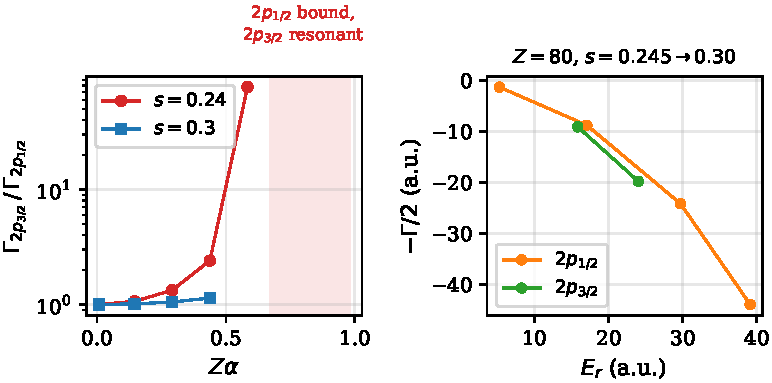
\includegraphics[width=\linewidth]{figures/figB_splitting.pdf}
\caption{Left: width ratio of the $2p$ fine-structure doublet vs.\
$\Za$ at fixed reduced screening $s=\lambda/Z$. Near threshold
($s=0.24$, red) the spin-symmetry breaking is amplified by orders of
magnitude and terminates in the shaded region where the $2p_{1/2}$ is
still bound while the $2p_{3/2}$ autoionizes; deep in the continuum
($s=0.30$, blue) the same doublet stays nearly symmetric. Right:
complex-plane trajectories of the doublet at $Z=80$ as the screening
sweeps $s=0.245\to0.30$; the $2p_{3/2}$ dissolves early while the
$2p_{1/2}$ traverses the fourth quadrant.}
\label{fig:splitting}
\end{figure}

Table~\ref{tab:prod} collects the production values for the $2p$
doublet ($\kappa=+1$: $2p_{1/2}$; $\kappa=-2$: $2p_{3/2}$) for $Z$ from
$1$ to $130$ at two reduced screenings, with grid spreads of
$10^{-11}$--$10^{-10}$ throughout. Figure~\ref{fig:splitting}
summarizes the physics.

\emph{Near-threshold amplification.} At $s=0.24$ the width ratio
$\Gamma_{2p_{3/2}}/\Gamma_{2p_{1/2}}$ grows monotonically:
$1.000$, $1.064$, $1.333$, $2.404$, $77.5$ for
$Z=1,20,40,60,80$. Beyond $Z\approx92$ the ratio is formally infinite:
the $2p_{1/2}$, whose critical screening exceeds $0.24$ in exactly this
range according to the bound-state map of Ref.~\cite{companionA},
remains bound while its fine-structure partner is a broad resonance.
The near-degeneracy of spin-doublet widths observed at high $\ell$ and
weak effective coupling~\cite{Shi2014} is thus completely broken in
the atomic strong-coupling regime.

\emph{A threshold effect.} At $s=0.30$, far above both thresholds, the
same doublet gives ratios of at most $1.14$ up to $Z=60$. The
amplification therefore does not reflect a uniformly growing
relativistic width shift: it is controlled by the distance of each
partner to \emph{its own} critical screening, to which the width is
exponentially sensitive. The splitting of the critical screenings
$\lambda_{c}(Z,\kappa)$ --- itself a purely relativistic, threshold-map
effect --- is transcribed into orders of magnitude in the widths near
threshold. Consistently, the resonances are born at the critical
screenings of the companion map: at $Z=40$, $\kappa=-2$ the
extrapolated birth point is $s_{c}=0.2207$ against the bound-state
value $0.216(4)$, and the width rises from threshold with the Wigner
$p$-wave law, measured exponent
$d\ln\Gamma/d\ln E_{r}=1.530$ against the theoretical $3/2$.

\emph{Sign inversion of the position splitting.} Near threshold
$E_{r}(2p_{3/2})>E_{r}(2p_{1/2})$, while deep in the continuum the
order reverses (at $Z=40$, $s=0.30$: $9.230$ vs.\ $8.979$). Splitting
inversions between different doublets were noted in the nuclear-style
cases of Ref.~\cite{Shi2014}; here a single doublet inverts between
regimes.

\begin{table}[t]
\caption{Production values for the $2p$ doublet of
$V=-Ze^{-\lambda r}/r$: $E_{r}$ and $\Gamma$ (a.u.), quoted at the
grid-spread precision ($\le10^{-10}$ unless noted). ``bound'' marks a
partner below its critical screening; ``dissolved'' a resonance too
broad for the $\theta\le0.8$ window. }
\label{tab:prod}
\begin{ruledtabular}
\begin{tabular}{llllll}
$Z$ & $s$ & \multicolumn{2}{c}{$2p_{1/2}$ ($\kappa=+1$)} &
\multicolumn{2}{c}{$2p_{3/2}$ ($\kappa=-2$)}\\
 & & $E_{r}$ & $\Gamma$ & $E_{r}$ & $\Gamma$\\
\colrule
1 & 0.24 & 0.002179006 & 0.002363910 & 0.002179167 & 0.002364262\\
1 & 0.30 & 0.005566663 & 0.018760420 & 0.005566558 & 0.018760950\\
20 & 0.24 & 0.840624043 & 0.878730 & 0.867171835 & 0.935150\\
20 & 0.30 & 2.247795246 & 7.406652 & 2.231161256 & 7.493011\\
40 & 0.24 & 2.941245536 & 2.711104 & 3.413196282 & 3.613002\\
40 & 0.30 & 9.229777734 & 28.37727 & 8.979248887 & 29.83296\\
60 & 0.24 & 4.598969039 & 3.181289 & 7.460504208 & 7.646312\\
60 & 0.30 & 21.50465234 & 58.52595 & 20.40804704 & 66.58487\\
80 & 0.24 & 0.848891758 & 0.159698 & 12.67315047 & 12.37604\\
80 & 0.30 & 39.11712762 & 87.92655 & \multicolumn{2}{c}{dissolved}\\
92 & 0.24 & \multicolumn{2}{c}{bound} & 16.13746549 & 15.16700\\
92 & 0.30 & 50.98258585 & 97.05267 & \multicolumn{2}{c}{dissolved}\\
110 & 0.24 & \multicolumn{2}{c}{bound} & 21.34539206 & 18.62827\\
110 & 0.30 & 60.90692212 & 77.12090 & \multicolumn{2}{c}{dissolved}\\
130 & 0.24 & \multicolumn{2}{c}{bound} & 26.14562678 & 20.34203\\
130 & 0.30 & \multicolumn{2}{c}{bound} & \multicolumn{2}{c}{dissolved}\\
\end{tabular}
\end{ruledtabular}
\end{table}

\section{Conclusions}

Two independent, mutually blind methods --- a certified complex-scaled
exact-structure discretization and Gamow shooting matched to exact free
spinors --- agree to ten--twelve digits on Dirac--Yukawa resonances,
turning the four-digit state of the art into benchmark tables,
correcting its narrow strong-coupling entries, and resolving widths
previously reported as zero. The physics outcome is a sharp statement
about relativistic symmetry in autoionization: the spin symmetry of
resonance widths, excellent at high angular momentum and away from
thresholds, is broken by orders of magnitude near the critical
screening, where the relativistic splitting of the thresholds
themselves is transcribed exponentially into the widths --- to the
point that one fine-structure partner autoionizes while the other
remains bound. The natural continuations are the $d$-doublets and the
supercritical finite-nucleus regime, and, on the methods side, the
finite-field problem where the same certified machinery meets
non-separable perturbations.

\begin{acknowledgments}
The author thanks the ESPOCH Faculty of Sciences for institutional
support. All scripts reproducing the tables and figures, including the
certification and verification batteries, are openly available with the
companion papers.
\end{acknowledgments}

\bibliography{refs}

\end{document}
